%!TEX root = ./template-skripsi.tex
%-------------------------------------------------------------------------------
%                            BAB II
%               KAJIAN TEORI
%-------------------------------------------------------------------------------

\chapter{KAJIAN PUSTAKA}

\section{Pengertian Klasifikasi Objek}

Fungsi dari klasifikasi objek adalah untuk memberikan deskripsi label ke 
sebuah segmentasi objek. Bila dilihat dari representasi fitur objek, ini 
dapat dicapai dengan melihat tanda-tanda keberadaan fitur yang mengindikasikan 
kelas dari objek. Hal ini umumnya dicapai dengan menentukan \textit{threshold} diantara 
kelas-kelas yang direpresentasikan oleh \textit{training set} yang sudah dilabeli. 
 Pelatihan otomatis umumnya mementingkan distribusi dari 
setiap kelas (distribusi harus setara), dan melabeli setiap contoh dengan benar, 
Namun, isu yang umum didalam cara ini pemilihan fitur-fitur yang akan digunakan untuk 
klasifikasi objek kadang kurang sesuai dan sering kali bergantung terhadap 
keberuntungan untuk mendapat hasil sangat akurat (\cite{rennoetal}).

\section{\emph{Viola Jones Object Detection Framework}}

Paul Viola dan Michael, J, Jones (\cite{rennoetal}) mempublikasikan sebuah makalah ilmiah dengan 
judul “\emph{Robust Real-Time Face Detection}”. Makalah tersebut mendeskripsikan sebuah 
framework pendeteksian wajah yang dapat memproses gambar secara cepat dengan 
tingkat akurasi yang tinggi. Ada tiga kontribusi penting dari makalah tersebut: 
Pertama adalah pengenalan sebuah representasi gambar baru yang dipanggil 
\emph{Integral Image} yang memungkinkan penghitungan fitur yang dipakai oleh detektor 
dilakukan dengan cepat. Yang kedua adalah sebuah classifier yang efisien dan 
sederhana, yang dibuat menggunakan algoritma pembelajaran \emph{Adaboost} 
(\cite{freundetal}) untuk memilih sejumlah fitur-fitur kritis dari 
fitur-fitur potensial. Yang ketiga adalah sebuah metode untuk menggabungkan 
fitur-fitur tersebut dalam sebuah bentuk \emph{cascade} yang memungkinakan algoritma 
untuk memfokuskan deteksi di area-area yang memiliki potensial saja.

\subsection{\emph{Features}}

\begin{figure}[H]
  \centering{}
	\includegraphics[width=0.6\textwidth]{gambar/haar\_features}
  \caption{Beberapa \emph{Haar-like features} yang digunakan framework Viola-Jones.}
\end{figure}

Ada banyak alasan dimana penggunaan fitur lebih baik daripada 
nilai piksel secara langsung. Alasan paling umum adalah fitur dapat berfungsi
untuk meng-\emph{encode ad-hoc domain knowledge} yang sulit dipelajari 
dengan jumlah data pelatihan yang terbatas. Untuk sistem \emph{framework Viola-Jones} 
ada alasan besar lainnya untuk penggunaan fitur yaitu sistem berbasis fitur beroperasi lebih cepat
daripada sistem yang berbasis nilai piksel.

Fitur sederhana yang digunakan mirip dengan \emph{Haar Basis Function} yang 
digunakan \cite{papaetal}. Lebih tepatnya ada tiga jenis fitur: dua persegi, tiga persegi dan 
empat persegi diagonal. 
Nilai dari sebuah \emph{fitur dua persegi} adalah perbedaaan diantara 
jumlah nilai piksel didalam dua atau lebih area persegi. Area-area tersebut memiliki 
ukuran dan bentuk yang sama, dan juga bersebelahan secara horizontal dan vertikal.
Subuah \emph{fitur tiga persegi} menghitung jumlah piksel dua area persegi 
di bagian luar dikurangi dengan jumlah nilai piksel persegi yang ada ditengah keduanya. 
Yang terakhir \emph{fitur empat persegi} menghitung perbedaan nilai dari dua pasang 
persegi diagonal.

% \subsection{\emph{Integral Image}}

% \begin{figure}[H]
%   \centering{}
% 	\includegraphics[width=0.6\textwidth]{gambar/integral\_image\_1}
%   \caption{Sebuah nilai \emph{Integral Image} $(x,y)$ dan area yang diwakilinyak}
% \end{figure}

% Fitur-fitur persegi dapat dihitung secara cepat menggunakan 
% representasi tidak langsung dari gambar, hal ini diberi nama 
% \emph{integral image}. \emph{integral image} pada lokasi $x, y$ berisikan 
% penjumlahan di atas dan di kiri dari $x, y$ dan nilai $x, y$ itu sendiri:
% \begin{equation}
%   i i(x, y)=\sum_{x^{\prime} \leq x, y^{\prime} \leq y} i\left(x^{\prime}, y^{\prime}\right),
% \end{equation}
% Dimana $ii(x,y)$ adalah \emph{integral image} dan $i(x,y)$ 
% adalah nilai piksel dari gambar aslinya. Menggunakan kedua 
% pengulangan berikut ini:
% \begin{equation}
%   s(x, y)=s(x, y-1) + i(x, y)
% \end{equation}
% \begin{equation}
%   ii(x, y)=ii(x-1, y) + s(x, y)
% \end{equation}
% (Dimana \emph{s(x, y)} adalah nilai kumulatif dari baris, \emph{s(x, -1) = 0}, 
% dan \emph{ii(-1, y) = 0}) \emph{Integral Image} dari sebuah gambar dapat dihitung dalam sekali jalan.

% \begin{figure}[H]
%   \centering{}
% 	\includegraphics[width=0.6\textwidth]{gambar/integral\_image\_2}
%   \caption{Jumlah dari intensitas cahaya pada persegi D dapat dihitung dengan 4 referensi \textit{array}. Nilai dari 1 adalah jumlah intensitas cahaya pada persegi A, Nilai dari 2 adalah persegi A + B, nilai dari 3 adalah A + C dan nilai 4 adalah A + B + C + D.}
% \end{figure}

% Menggunakan \emph{integral image}, semua jumlah nilai pada persegi dapat 
% dihitung didalam 4 referensi \emph{array}. Jelas perbedaan 
% diantara kedua jumlah nilai-nilai persegi dapat dihitung 
% dengan delapan referensi. Karena peresegi dua fitur yang 
% didefinisikan diatas melibatkan juga nilai persegi disebelahnya, 
% mereka dapat dikomputasi dengan enam referensi \emph{array}, delapan referensi
% bilamana ia adalah persegi tiga fitur, dan sembilan referensi untuk 
% persegi empat fitur.

% Kecepatan yang didapat dari penghitungan \emph{Integral Image} ini dapat dijustifikasi 
% bila kita membandingkannya dengan perhitungan manual. Sebagai contoh, misalkan 
% kita sedang mencari jumlah total intensitas cahaya pada ukuran area 10x10 
% piksel. Cara manual mengharuskan kita menghitung sampai 100 kali untuk mendapat 
% jumlah intensitas cahaya pada area tersebut, belum lagi proses ini harus 
% diulang terus-menerus untuk ukuran dan lokasi yang berbeda. Dilain sisi, 
% perhitungan menggunakan \emph{Integral Image} hanya perlu mereferensi tabel yang 
% sudah dibuat sebelum semua usaha klasifikasi, dalam hal ini kita hanya perlu 
% melakukan perhitungan empat kali untuk menghitung intensitas cahaya dalam area 
% tersebut.

\subsection{\emph{Adaboost}}

\begin{algorithm}
\caption{SAMME Adaboost Algorithm}
\begin{algorithmic}[1]
\State \textbf{Input:} Set latihan $\{(x_i, y_i)\}_{i=1}^N$ dimana $x_i$ adalah sampel ke-$i$ dan $y_i$ adalah labelnya, jumlah \textit{weak classifiers} $M$
\State \textbf{Output:} Urutan \textit{classifier} $H(x)$
\State Inisiasi bobot gambar: $w_i^{(1)} = \frac{1}{N}, i=1,2,\ldots,N$
\For{$m=1$ to $M$}
    \State latih \textit{weak classifier} $h_m(x)$ dengan distribusi $w_i^{(m)}$
    \State Hitung error pada klasifikasi: $\epsilon_m = \sum_{i=1}^N w_i^{(m)} \cdot \text{I}(h_m(x_i) \neq y_i)$
    \State Hitung bobot \textit{weak classifier}: $\alpha_m = \frac{1}{2} \log\left(\frac{1 - \epsilon_m}{\epsilon_m}\right)$
    \State Ubah bobot gambar sesuai error pada klasifikasi:
    \State \hspace{\algorithmicindent} For $i=1,2,\ldots,N$: $w_i^{(m+1)} = w_i^{(m)} \cdot \exp(-\alpha_m \cdot \text{I}(h_m(x_i) \neq y_i))$
    \State Normalisasi bobot gambar: $w_i^{(m+1)} = \frac{w_i^{(m+1)}}{\sum_{i=1}^N w_i^{(m+1)}}$
\EndFor
\State Hasil \textit{strong classifier}: $H(x) = \text{sign}\left(\sum_{m=1}^M \alpha_m \cdot h_m(x)\right)$
\end{algorithmic}
\end{algorithm}

Dalam \emph{framework Viola-Jones} sebuah varian dari \emph{Adaboost} 
digunakan untuk memilih fitur dan juga untuk melatih \textit{classifier}. 
Didalam bentuk aslinya, algoritma pembelajaran \emph{Adaboost} digunakan 
untuk mem-\textit{boost} performa klasifikasi dari algoritma pembelajaran 
sederhana. \emph{Adaboost} melakukan ini dengan menggabungkan sekumpulan 
\emph{classifier} lemah untuk membuat sebuah \emph{classifier} kuat. 
Didalam istilah \emph{Boosting}, \emph{classifier} lemah disebut juga 
dengan \emph{weak learner}. Sebagai contoh, algoritma pembelajaran \emph{perceptron} 
mencari dari sekelompok \emph{perceptron} dan mengambil \emph{perceptron} 
dengan tingkat kesalahan klasifikasi terendah. Algoritma pembelajaran disebut 
lemah karena kita tidak berharap \emph{classifier} terbaik untuk mengklasifikasi 
data dengan benar. Nyatanya, \emph{perceptron} terbaik mungkin 
hanya memiliki tingkat akurasi 51\%. Agar \emph{weak learner} dapat di-\textit{boost}, 
ia akan dipanggil untuk menyelesaikan sederet problem pembelajaran. Setelah 
satu ronde pembelajaran selesai, setiap contoh pembelajarannya akan dibobot ulang 
untuk menekankan problem yang salah diklasifikasi oleh \emph{weak learner} 
sebelumnya. Bentuk \emph{final strong classifier} adalah 
sebuah kombinasi \emph{weak learner} berbobot. 

\subsection{\emph{Weaklearn}}

\begin{algorithm}
  \caption{Metode Pembuatan \textit{Decision Tree}}
  \begin{algorithmic} [1]
    \State Anotasi semua dataset sesuai kelasnya. \textit{Decision Tree} lalu 
    akan dimulai dari akar
    \State Pilih atribut terbaik untuk melakukan \textit{split} dengan melakukan 
    \emph{Information Gain} (IG):
    \begin{equation}
      IG(S, A) = Entropi(S) - sum_v \frac{S_v}{S} x Entropi(S_v)
    \end{equation} 
    dimana:
    \begin{itemize}
      \item $S$: kumpulan sampel pada \emph{node} sekarang
      \item $A$: atribut yang digunakan untuk \textit{split}
      \item $v$: Sebuah nilai atribut $A$ yang membagi $S$ menjadi turunan $S_v$
      \item Entropi($S$) = $-sum_c p_c log_2(p_c)$: Ukuran kemurnian pada kumpulan 
      contoh dengan target label. Dimana $p_c$ adalah proporsi contoh $S$ yang ada 
      pada kelas $c$. 
    \end{itemize}
    %Masukin IGR kalo perlu (Information Gain Ratio)
    \State \textit{split} pohon ke \textit{node} turunan sesuai atribut yang dipilih 
    \State tentukan apabila seluruh contoh sudah jatuh ke kelas yang benar(\textit(information gain) = 0) 
    atau tidak bila tinggi maksimum sudah dicapai, bila tidak 
    maka ulangi langkah 2 dan 3.
  \end{algorithmic}
\end{algorithm}

\emph{Framework Viola Jones} menggunakan sebuah \emph{weaklearn} yang bernama 
\emph{Decision Stump}, atau sebuah \emph{Decision Tree} yang hanya memiliki 
dua daun kelas saja. \emph{Decision Tree} sendiri mampu digunakan untuk 
permasalahan \emph{multi-class}.

\emph{Decision Tree} menghasilkan sebuah classifier didalam bentuk sebuah pohon 
pilihan, sebuah struktur yang berbentuk:
\begin{itemize}
  \item Sebuah daun, mengindikasi sebuah kelas, atau
  \item Sebuah \emph{decision node} yang menspesifikasi 
  sebagian tes untuk dikerjakan atas sebuah nilai 
  atribut, dengan satu \emph{branch} dan \emph{subtree} untuk 
  setiap hasil dari tes.
\end{itemize}

Sebuah \emph{Decision Tree} dapat digunakan untuk mengkasifikasi sebuah kasus 
dengan memulai dari akar pohon dan bergerak sampai sebuah daun ditemukan. 
Pada setiap \emph{node} yang bukan merupakan daun, hasil dari tes kasus 
dideterminasi dan tes berlanjut ke \emph{node} berikutnya sesuai dengan 
hasil tes tersebut. Ketika proses pada akhirnya (dan dengan pasti) 
menuju ke sebuah daun, kelas dari kasus diprediksi sesuai label yang ada pada daun.

% \subsection{\emph{Boosting}}

% \emph{Boosting} adalah sebuah metode didalam ilmu komputer, yang digunakan untuk 
% meningkatkan performa sekelompok \textit{weak learn} dengan menyatukan mereka menjadi 
% sebuah \textit{strong classifier}. Hal ini dilakukan dengan cara mengiterasi sederet 
% \textit{weak classifier} untuk menyelesaikan sebuat set data dan memberikan mereka 
% bobot voting. Sebuah \textit{weak classifier} 
% pertama memprediksi kelas dari sebuah set contoh data, yang kemudian hasilnya akan dibandingkan 
% dengan label yang seseungguhnya. Contoh yang gagal diprediksi oleh \textit{weak classifier} 
% yang pertama lalu akan dicatat dan akan ditingkatkan bobot nilainya, jadi \textit{weak classifier} 
% berikutnya bisa mendapatkan nilai lebih bila berhasil mengklasifikasi contoh tersebut dengan benar. 
% proses ini dijalankan hingga \textt{weak classifier} habis, dan dimulai lagi bila ditemukan 
% bahwa hasil prediksi akhir meningkat daripada iterasi sebelumnya.

\subsection{\emph{Attentional Cascade}}

\begin{figure}[H]
  \centering{}
	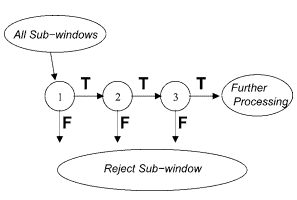
\includegraphics[width=0.6\textwidth]{gambar/cascade}
  \caption{\textit{Workflow} dari \emph{Attentional Cascade}}
\end{figure}

\emph{Attentional Cascade} adalah sebuah \emph{cascade} dari banyak 
\emph{classifier} yang dibuat untuk meningkatkan performa deteksi dengan secara radikal mengurangi jumlah 
komputasi. Intinya \emph{weak classifier} yang telah di-\emph{boost} dapat dibuat lebih 
kecil dan efisien, yang dapat menolak mayoritas \emph{sub-window} negatif dan 
mendeteksi sebagian besar dari \emph{sub-window} positif. \emph{Classifier} yang lebih 
sederhana digunakan untuk menolak mayoritas \emph{sub-window} sebelum \emph{classifier} 
yang lebih kompleks dipanggil untuk menurunkan tingkat \emph{false positives}.

Struktur dari \emph{cascade} merefleksikan 
fakta bahwa pada gambar apapun mayoritas \emph{sub-window} pasti negatif. 
Oleh karena itu, \emph{cascade} berusaha untuk sebanyaknya menolak sub-window 
negatif pada tahapan seawal mungkin. Sementara hasil positif 
akan memicu evaluasi dari setiap \emph{classifier} dalam \emph{cascade}, 
hal ini sangatlah langka.

Layaknya sebuah \emph{Decision Tree}, sebuah \emph{classifier} dilatih menggunakan 
contoh-contoh yang telah berhasil melewati tahap sebelumnya. Oleh karenanya, 
\emph{classifier} pada tahap kedua menghadapi tantangan yang jauh lebih sulit 
daripada yang pertama.

\emph{Cascade} dimulai dengan membuat sebuah \textit{stage} awal, dimana \textit{weak classifier} 
ditambahkan secara perlahan hingga \emph{detection rate} yang dituju sampai. \emph{Detection rate} 
ini harus disesuaikan oleh pengguna sesuai dengan keperluannya, tujuannya tetap untuk mengurangi 
waktu komputasi tapi juga mencoba agar tidak terlalu banyak kasus \emph{false positive} yang dapat 
lewat.

% \begin{algorithm}
%   \caption{Algoritma Pelatihan Untuk Pembuatan \textit{Cascaded Detector}}
%   \begin{algorithmic} [1]
%     \State Pengguna memilih nilai dari \textit{f}, nilai maksimum \emph{false positive} 
%     pada setiap tahap yang dapat diterima, dan \textit{d}, nilai minimum \emph{detection rate} 
%     per tahap yang dapat diterima
%     \State Pengguna memilih target keseluruhan \emph{false positive rate}, $F_{target}$
%     \State \textit{P} = kumpulan contoh positif
%     \State \textit{N} = kumpulan contoh negatif
%     \State $F_0 = 1.0; D_0 - 1.0$
%     \State $i = 0$
%     \State $while F_i > F_{target}$
%     \Statex $-i \leftarrow i + 1$
%     \Statex $-n_i = 0; F_i = F_i-_1$
%     \Statex -while $F_i > f x F_i-_1$
%     \begin{itemize}
%       \item $n_i \leftarrow n_i + 1$
%       \item Gunakan \textit{P} dan \textit{N} untuk melatih sebuah \emph{classifier}
%       dengan fitur $n_i$ menggunakan \emph{Adaboost} 
%       \item Evaluasi \emph{cascade classifier} dengan \textit{set} validasi
%       untuk menentukan $F_i$ dan $D_i$. 
%       \item kurangi \textit{threshold} untuk \emph{classifier} ke-$i$ sampai 
%       \emph{cascade classifier} memiliki tingkat deteksi paling tidak $d x D_i-_1$ 
%       (hal ini juga akan mempengaruhi $F_i$)
%     \end{itemize}
%     \Statex $-N \leftarrow$ {\O}
%     \Statex -if $F_i > F_target$ evaluasi \emph{cascade detector} menggunakan 
%     \textit{set} negatif dan masukan semua deteksi gagal ke \textit{set} N
%   \end{algorithmic}
% \end{algorithm}

